\chapter{А так звучит красиво? Гармоничность}
\label{ch:harmony}


\section{Сколько вешать в полутонах? Интервалы}
\label{ch:harmony:interval}

\begin{Definition}[Интервал]
    \emph{Интервал} --- это расстояние между \emph{двумя} звуками, выраженное в полутонах. 
\end{Definition}

Это определение для математиков. Для музыкантов же интервалы \emph{звучат}! Если два звука прозвучали одновременно, то интервал называется гармоническим, а если друг за другом --- мелодическим.

\begin{Example}[Послушаем гармонические интервалы]
    \label{ex:harmony:interval:string5and6}
    Возьмите настроенную гитару. Поиграем на 5 и 6-й струне. Если гитара настроена страндартно, то 6-я струна на 5-м ладу прозвучит в унисон с открытой 5-й струной. Такое расстояние в 0 полутонов музыканты называют \emph{примой}. 
    
    Теперь расслабьтесь, успокойтесь, забудьте обо всех горестях и радостях. Сосредоточьтесь на своем дыхании. Существует только ваше дыхание. Абсолютный покой. 
    
    Не получается? Черт с ним!
    
    Зажимаем 6-ю струну на 5-м ладу и одновременно играем две струны 6-ю и 5-ю. Даем позвучать, прислушиваемся к ощущениям.
    
    И так далее, двигаясь по 6-й струне: 6-й лад, 7, 8, 9, 10, 11, 12, 13, 14, 15, 16, 17. Играем две струны, всякий раз прислушиваемся к ощущениям.
\end{Example}

Интервал, приятный на слух музыканты называют \emph{консонансом}, а неприятный --- \emph{диссонансом}. 

Чтобы разобраться в том, почему звучание одного интервала нам нравится, а другого --- нет, визуализируем результат наложения двух звуков. Пусть функция $\sin(x)$ изображает основной тон исходного звука. Функция $\sin(x\cdot(\sqrt[12]{2})^n)$ будет изображать звук, который \emph{выше} исходного на $n$ \emph{полутонов}. Результату совместного звучания будет соответствовать их сумма\footnote{В Интернете масса сайтов, позволяющих построить график функции. Более того, просто вбейте в гугл \texttt{sin(x)+sin(x*(2\^{}(1/12)))} и дивитесь чудесам Технологии!}:
\begin{equation}
    \label{eq:harmony:interval:sin}
    \sin(x) + \sin(x\cdot(\sqrt[12]{2})^n).
\end{equation}

Результаты построения графиков совместного звучания (построен красным цветом) на фоне исходного звука (синий цвет) для интервалов от $n=1$ до $n=11$ полутонов (т.е. в рамках октавы) приведены в таблицах \ref{t:harmony:interval:disso-1-2-10-11}, \ref{t:harmony:interval:conso-3-4-8-9}, \ref{t:harmony:interval:conso-5-7}, \ref{t:harmony:interval:disso-6}.


Итак, диссонансы приведены в таблице \ref{t:harmony:interval:disso-1-2-10-11}. Вам не должны были понравиться интервалы на 6,7,15,16 ладах 6-й струны, если вы проходили пример \ref{ex:harmony:interval:string5and6}. Только не говорите, что понравились! Пора сходить к доктору!!! Не затягивайте.

\begin{table}[!ht]
    \caption{Диссонансы в графиках функции \ref{eq:harmony:interval:sin}}
    \label{t:harmony:interval:disso-1-2-10-11}
    \centering
    \begin{tabular}{c|c}
        \hline\hline
        1 полутон, $n=1$        & 2 полутона, $n=2$ \\
        малая секунда           & большая секунда \\
        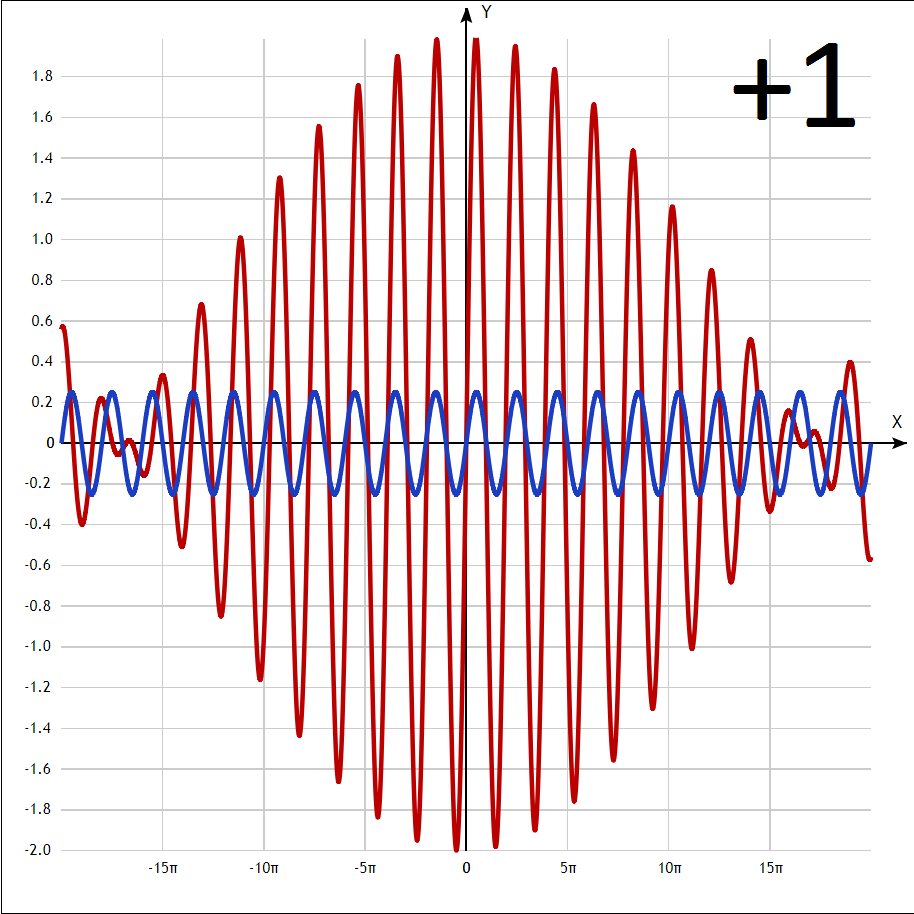
\includegraphics[width=0.45\textwidth]{fig/intervals/i01}
            & 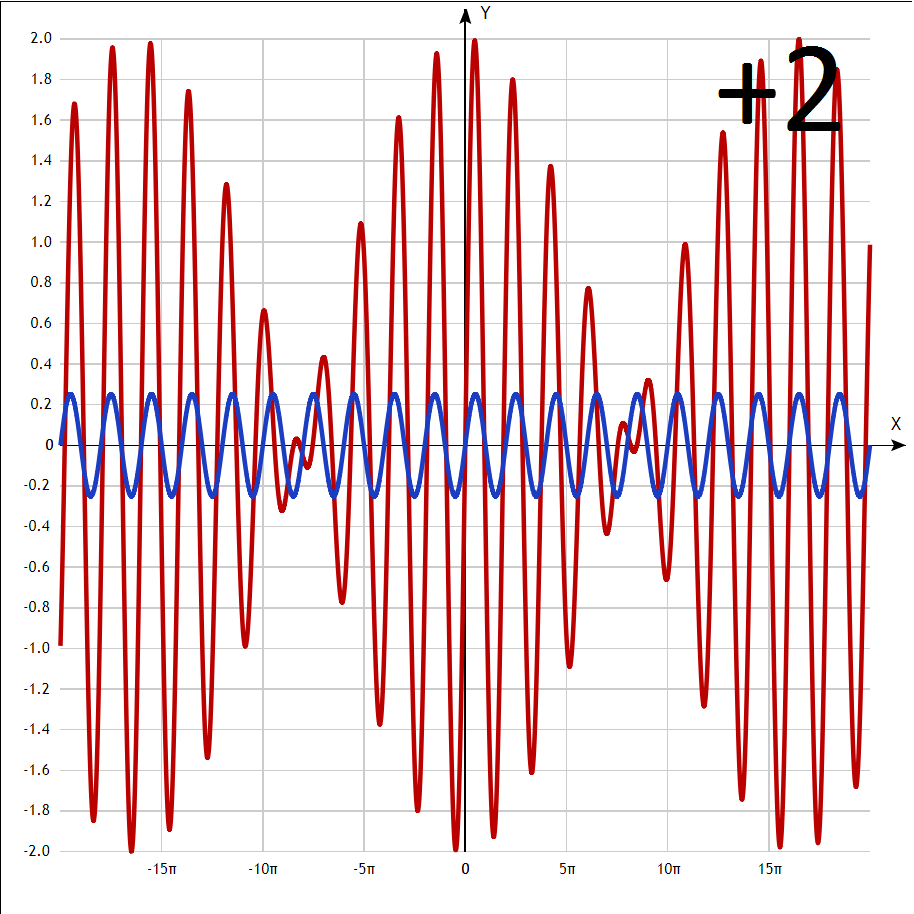
\includegraphics[width=0.45\textwidth]{fig/intervals/i02} \\
        \hline\hline
        10 полутонов, $n=10$    & 11 полутонов, $n=11$ \\
        малая септима           & большая септима \\
        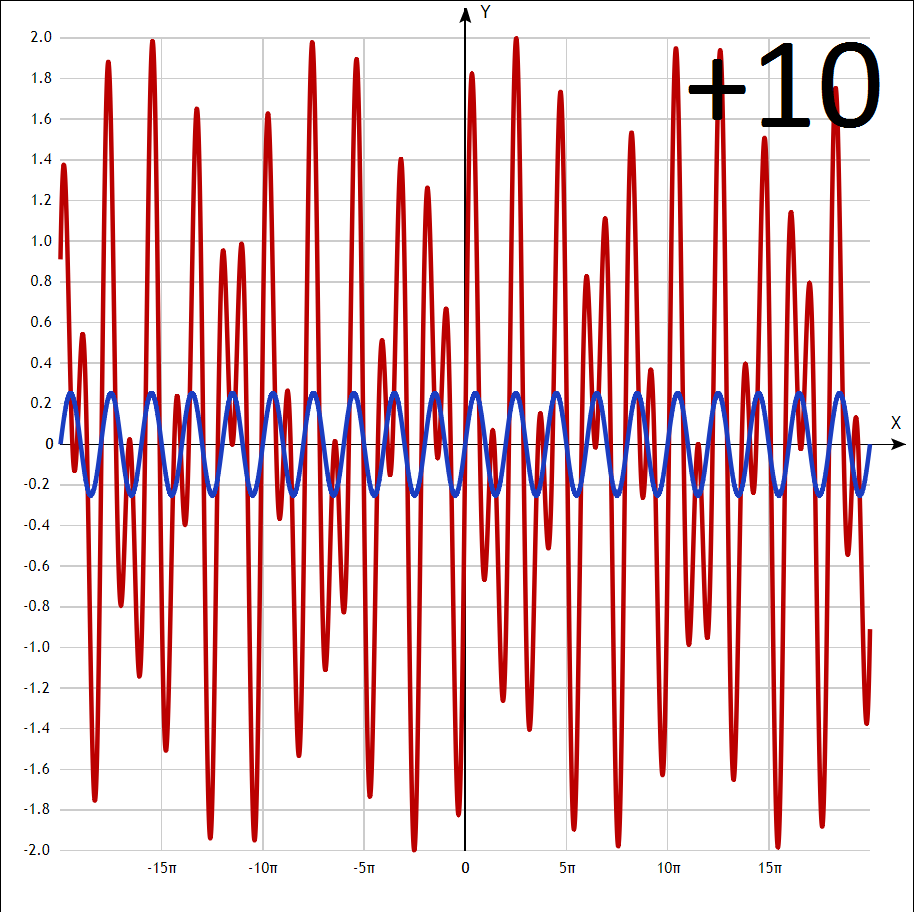
\includegraphics[width=0.45\textwidth]{fig/intervals/i10}
            & 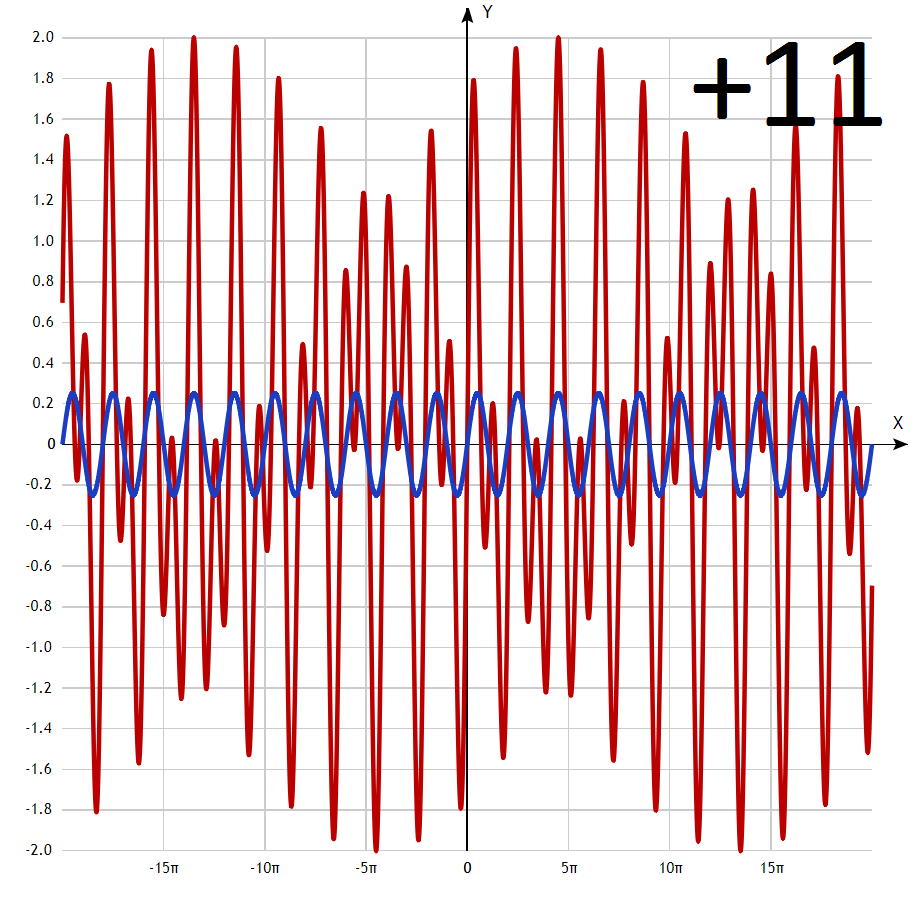
\includegraphics[width=0.45\textwidth]{fig/intervals/i11} \\
        \hline\hline
    \end{tabular}
\end{table}

Проанализируйте приведенные графики и попробуйте самостоятельно сделать выводы об особенностях консонансов и диссонансов. Стоит отметить, что принято также разделять совершенные и несовершенные консонансы. 

\begin{table}[!ht]
    \caption{Несовершенные консонансы в графиках функции \ref{eq:harmony:interval:sin}}
    \label{t:harmony:interval:conso-3-4-8-9}
    \centering
    \begin{tabular}{c|c}
        \hline\hline
        3 полутона, $n=3$   & 4 полутона, $n=4$ \\
        малая терция        & большая терция \\
        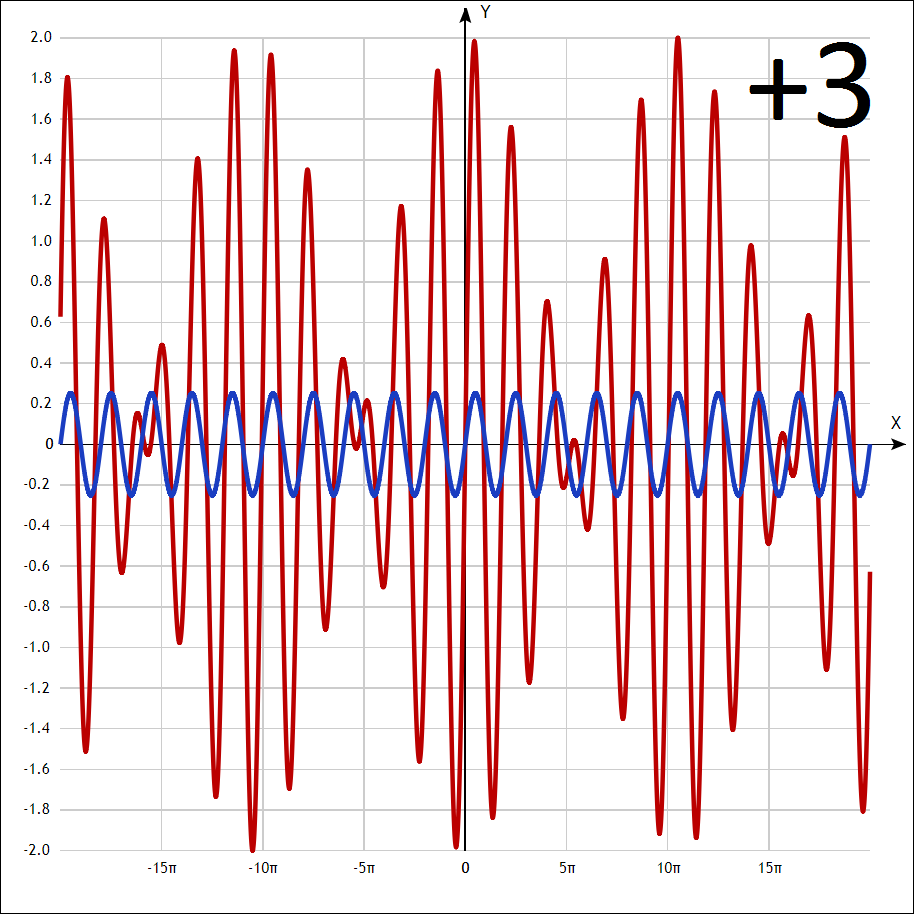
\includegraphics[width=0.45\textwidth]{fig/intervals/i03}
            & 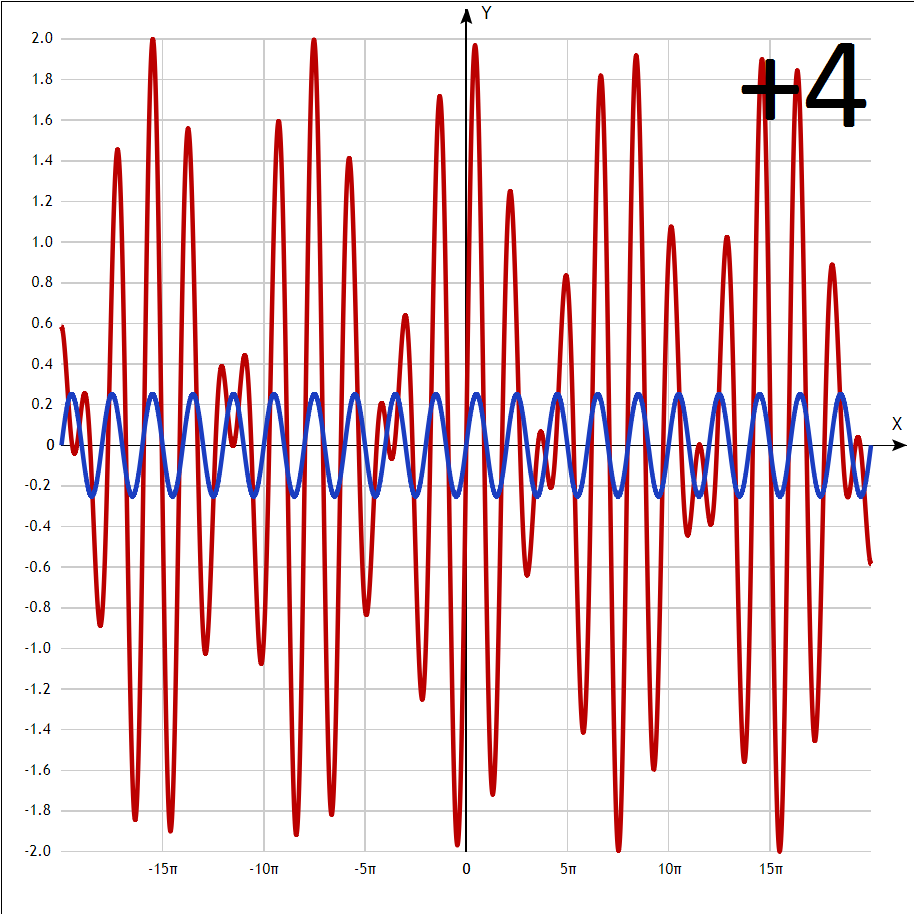
\includegraphics[width=0.45\textwidth]{fig/intervals/i04} \\
        \hline\hline
        8 полутонов, $n=8$  & 9 полутонов, $n=9$ \\
        малая секста        & большая секста \\
        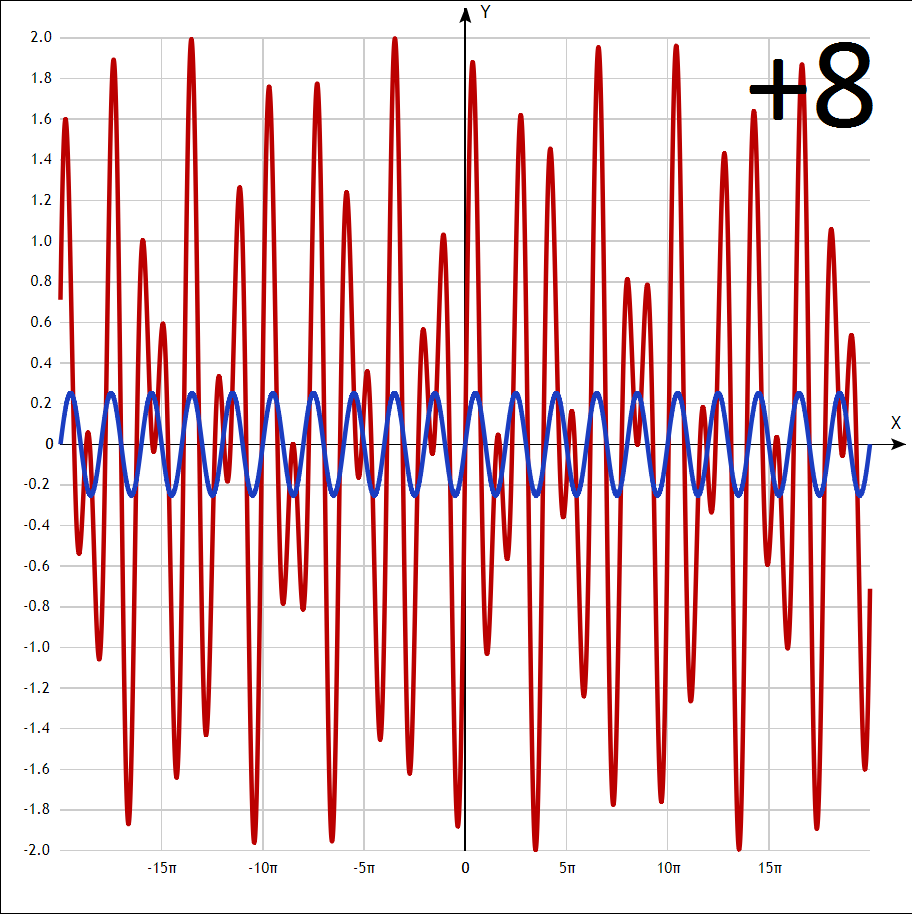
\includegraphics[width=0.45\textwidth]{fig/intervals/i08}
            & 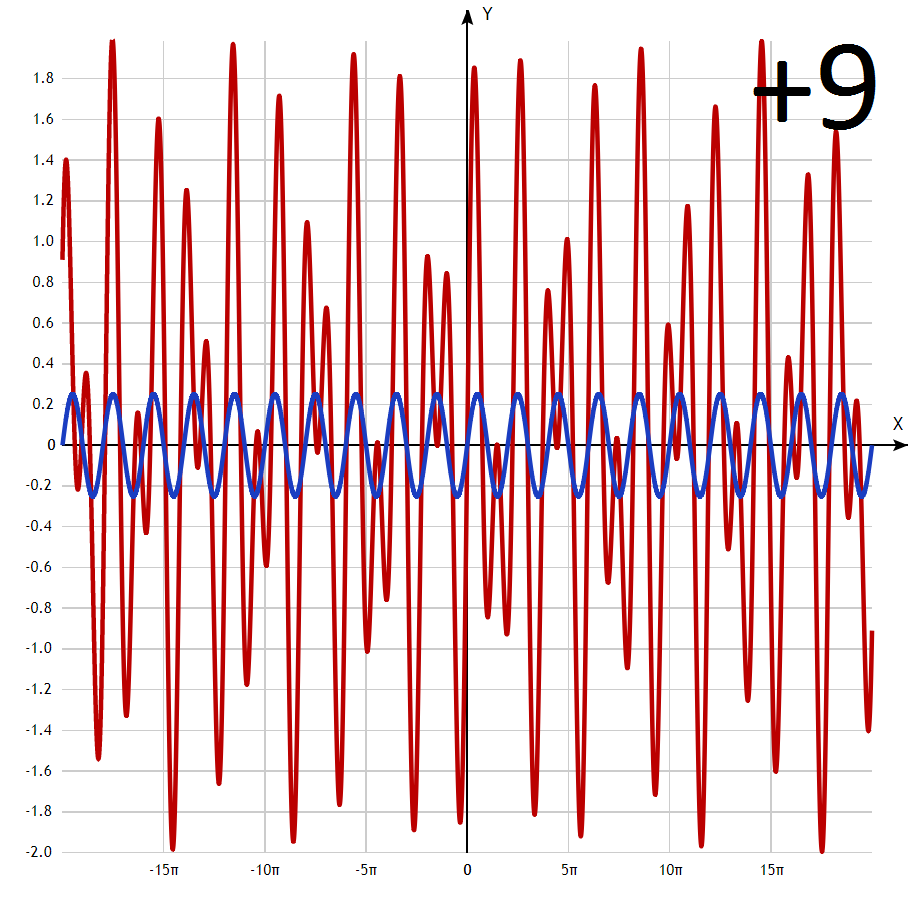
\includegraphics[width=0.45\textwidth]{fig/intervals/i09} \\
        \hline\hline
        
    \end{tabular}
\end{table}

\begin{table}[!ht]
    \caption{Совершенные консонансы в графиках функции \ref{eq:harmony:interval:sin}}
    \label{t:harmony:interval:conso-5-7}
    \centering
    \begin{tabular}{c|c}
        \hline\hline
        5 полутонов, $n=5$  & 7 полутонов, $n=7$ \\
        чистая кварта       & чистая квинта \\
        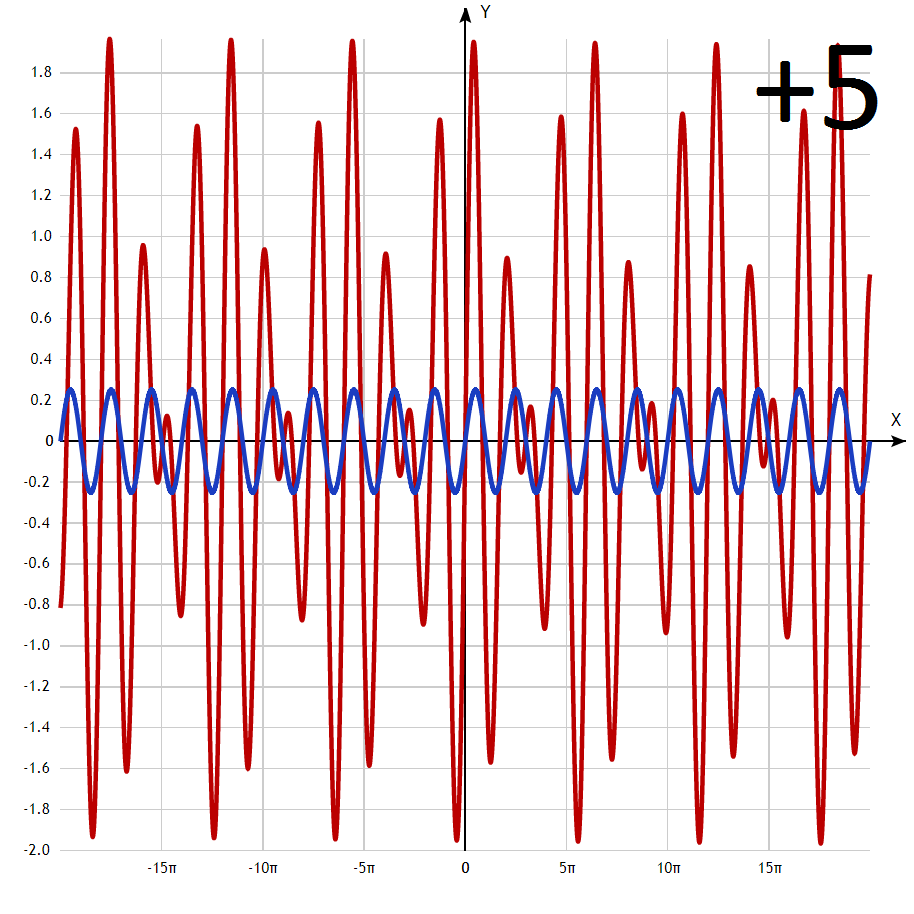
\includegraphics[width=0.45\textwidth]{fig/intervals/i05} 
            & 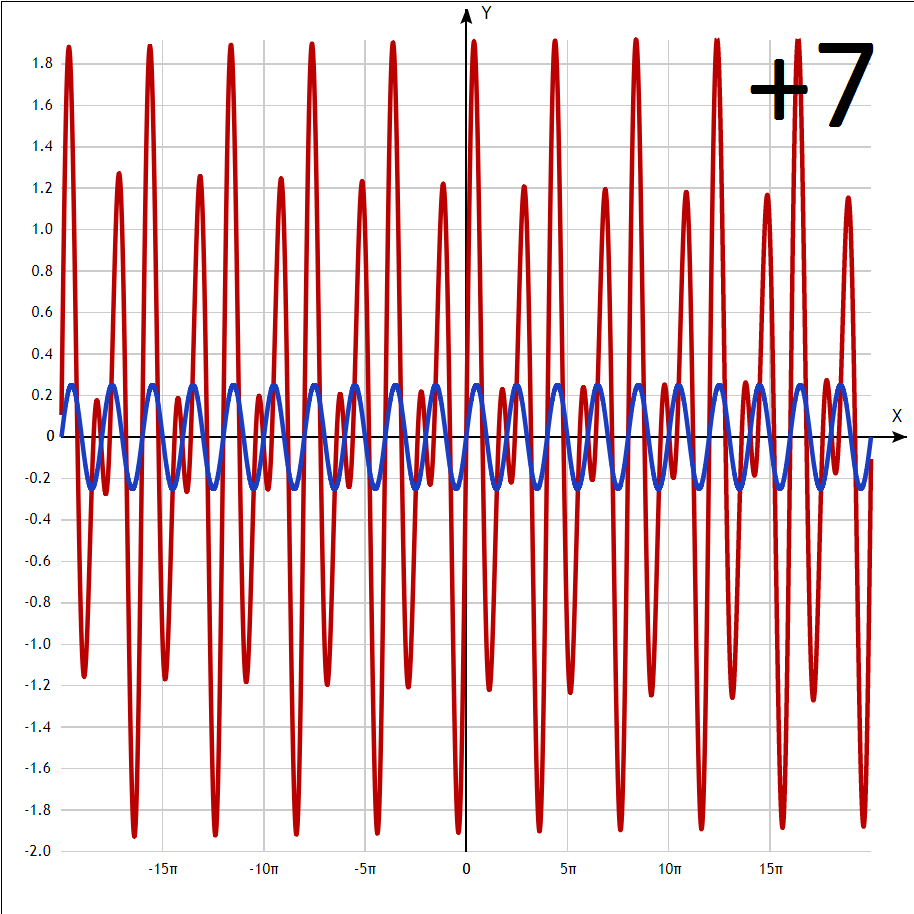
\includegraphics[width=0.45\textwidth]{fig/intervals/i07} \\
        \hline\hline
    \end{tabular}
\end{table}

\begin{table}[!ht]
    \caption{Диссонанс в графике функции \ref{eq:harmony:interval:sin}}
    \label{t:harmony:interval:disso-6}
    \centering
    \begin{tabular}{c}
        \hline\hline
        6 полутонов, $n=6$ \\
        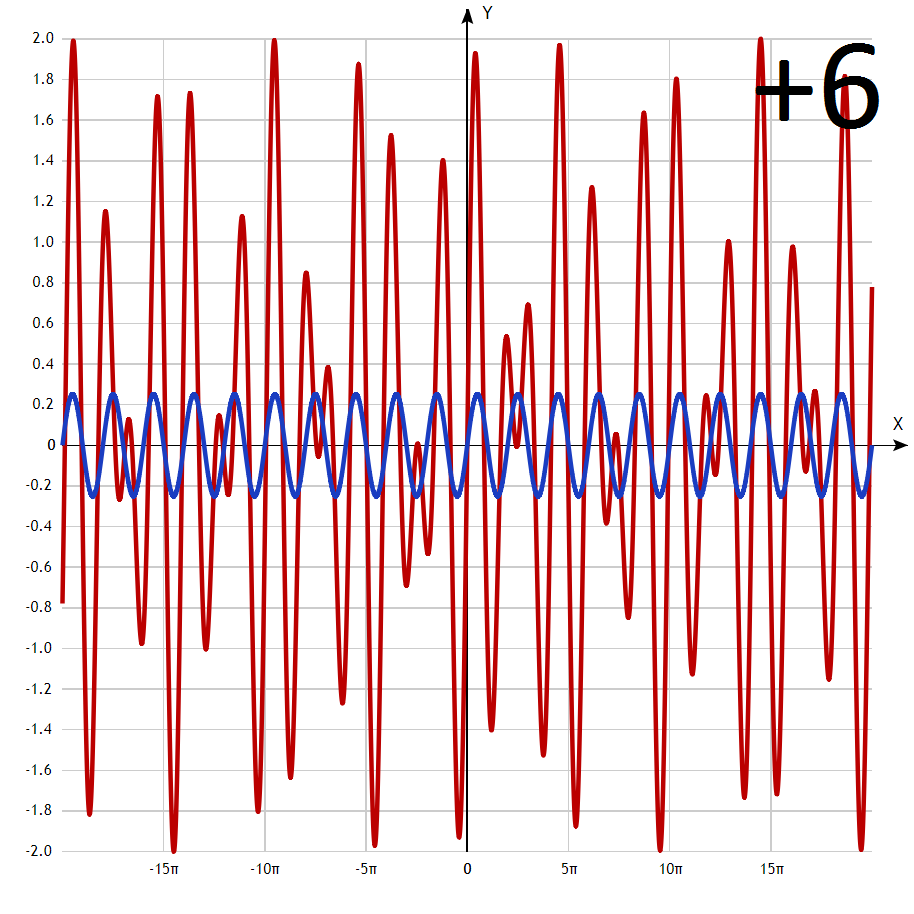
\includegraphics[width=0.45\textwidth]{fig/intervals/i06} \\
        увеличенная кварта,\\
        она же --- уменьшенная квинта,\\
        он же --- тритон\\
        \hline\hline
    \end{tabular}
\end{table}


\section{Лады? Лады}
\label{ch:harmony:lad}


\section{Чем больше, тем лучше? Аккорды}
\label{ch:harmony:chords}

